\documentclass[tikz]{standalone}

% Font
\usepackage{mathpazo}
\usepackage{libertine}
\renewcommand*\sfdefault{phv}

\large

% Color
\usepackage{xcolor}
\definecolor{f1}{HTML}{F39019}
\definecolor{b1}{HTML}{DE6A10}
\definecolor{f2}{HTML}{51A7F9}
\definecolor{b2}{HTML}{0365C0}
\definecolor{f3}{HTML}{70BF41}
\definecolor{b3}{HTML}{00882B}

% tikz
\usepackage{tikz}
\tikzstyle{every node}=[font=\sffamily]
\usetikzlibrary{shapes,arrows,positioning,calc,decorations.markings,backgrounds}
\tikzstyle{c1} = [thick,draw=b1,fill=f1]
\tikzstyle{c2} = [thick,draw=b2,fill=f2]
\tikzstyle{c3} = [thick,draw=b3,fill=f3]
\tikzstyle{cg} = [thick,draw=gray!50,fill=gray!30]
\tikzstyle{rect} = [rectangle, minimum height=1cm]
\tikzstyle{roundrect} = [rect, rounded corners=.2cm]
\tikzstyle{io} = [trapezium, trapezium left angle=70, trapezium right angle=110]
\tikzstyle{arrow} = [thick,->,>=stealth]
\tikzstyle{rect} = [fill=gray!40, minimum width=1.2cm, minimum height=.7cm]
\tikzstyle{new} = [fill=f2!40]
\tikzstyle{border} = [draw=black, dashed]
\tikzstyle{nc} = [circle, minimum size=.4cm, scale=.5, fill=black, opacity=.5]
\tikzstyle{oc} = [circle, minimum size=.4cm, scale=.5, fill=b1, opacity=.5]
\tikzstyle{uc} = [circle, minimum size=.4cm, scale=.5, fill=b2, opacity=.5]
\tikzstyle{next} =[single arrow, fill=f3!60, text width=.5cm, text height=.05cm, single arrow head extend=.12cm]
\tikzset{cross/.style={cross out, draw=black, minimum size=2*(#1-\pgflinewidth), inner sep=0pt, outer sep=0pt},
	%default radius will be 1pt. 
	cross/.default={1pt}}

\begin{document}
	
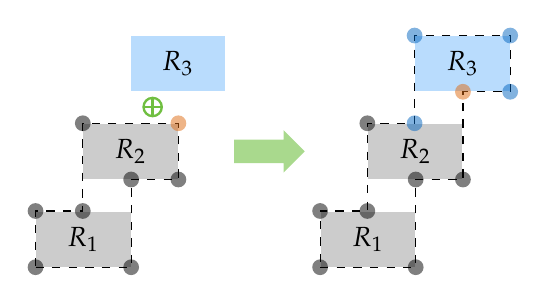
\begin{tikzpicture}
	
\node (r1) [rect] {$R_1$};
\node (r2) [rect, above=.4 of r1, xshift=.6cm] {$R_2$};
\node (r3) [rect, new, above=.4 of r2, xshift=.6cm] {$R_3$};

% dash border
\path[border] let \p1=(r1.north east), \p2=(r2.south west) in 
(r1.south west) node[nc]{}
-- (r1.south east) node[nc]{}
-- (\x1, \y2) node[nc]{}
-- (r2.south east) node[nc]{}
-- (r2.north east) node[oc]{}
-- (r2.north west) node[nc]{}
-- (\x2, \y1) node[nc]{}
-- (r1.north west) node[nc]{}
-- cycle;

% merge operator
\draw node[cross=3pt,f3,above=.15 of r2, line width=.3mm, xshift=.33cm,rotate=45]{};
\draw node [circle, above=.08 of r2, draw=f3, line width=.3mm, scale=.7, xshift=.4cm] {};

\node (arr) [next, right=.7 of r2] {};

\node (r1) [rect, right=2.4 of r1] {$R_1$};
\node (r2) [rect, above=.4 of r1, xshift=.6cm] {$R_2$};
\node (r3) [rect, new, above=.4 of r2, xshift=.6cm] {$R_3$};

% dash border
\path[border] let \p1=(r1.north east), \p2=(r2.north east), \p4=(r2.south west) , \p3=(r3.south west) in 
(r1.south west) node[nc]{}
-- (r1.south east) node[nc]{}
-- (\x1, \y4) node[nc]{}
-- (r2.south east) node[nc]{}
-- (\x2, \y3) node[oc]{}
-- (r3.south east) node[uc]{}
-- (r3.north east) node[uc]{}
-- (r3.north west) node[uc]{}
-- (\x3, \y2) node[uc]{}
-- (r2.north west) node[nc]{}
-- (\x4, \y1) node[nc]{}
-- (r1.north west) node[nc]{}
-- cycle;
	
\end{tikzpicture}
	
\end{document}